\documentclass[12pt,b5paper]{ltjsarticle}

%\usepackage[margin=15truemm, top=5truemm, bottom=5truemm]{geometry}
%\usepackage[margin=10truemm,left=15truemm]{geometry}
\usepackage[margin=10truemm]{geometry}

\usepackage{amsmath,amssymb}

% 定理環境
%\usepackage{amsthm}
%\newtheorem{theo}{Theorem}

%\pagestyle{headings}
\pagestyle{empty}

%\usepackage{listings,url}
%\renewcommand{\theenumi}{(\arabic{enumi})}

%\usepackage{graphicx}

\usepackage{tikz} % https://jp.mirrors.cicku.me/ctan/graphics/pgf/base/doc/pgfmanual.pdf
%\usetikzlibrary {arrows.meta}

%\usepackage{wrapfig}
%\usepackage{bm}

% ルビを振る
\usepackage{luatexja-ruby}

%% 核Ker 像Im Hom を定義
\newcommand{\Ker}{\mathop{\mathrm{Ker}}\nolimits}
%\newcommand{\Img}{\mathop{\mathrm{Im}}\nolimits}
\newcommand{\Ran}{\mathop{\mathrm{Ran}}\nolimits}
%\newcommand{\Hom}{\mathop{\mathrm{Hom}}\nolimits}

%\DeclareMathOperator{\Rot}{rot}
%\DeclareMathOperator{\Div}{div}
%\DeclareMathOperator{\Grad}{grad}
%\DeclareMathOperator{\arcsinh}{arcsinh}
%\DeclareMathOperator{\arccosh}{arccosh}
%\DeclareMathOperator{\arctanh}{arctanh}

\usepackage{url}

%\usepackage{listings}
%
%\lstset{
%%プログラム言語(複数の言語に対応,C,C++も可)
%  language = Python,
%%  language = Lisp,
%%  language = C,
%  %背景色と透過度
%  %backgroundcolor={\color[gray]{.90}},
%  %枠外に行った時の自動改行
%  breaklines = true,
%  %自動改行後のインデント量(デフォルトでは20[pt])
%  breakindent = 10pt,
%  %標準の書体
%%  basicstyle = \ttfamily\scriptsize,
%  basicstyle = \ttfamily,
%  %コメントの書体
%%  commentstyle = {\itshape \color[cmyk]{1,0.4,1,0}},
%  %関数名等の色の設定
%  classoffset = 0,
%  %キーワード(int, ifなど)の書体
%%  keywordstyle = {\bfseries \color[cmyk]{0,1,0,0}},
%  %表示する文字の書体
%  %stringstyle = {\ttfamily \color[rgb]{0,0,1}},
%  %枠 "t"は上に線を記載, "T"は上に二重線を記載
%  %他オプション:leftline,topline,bottomline,lines,single,shadowbox
%  frame = TBrl,
%  %frameまでの間隔(行番号とプログラムの間)
%  framesep = 5pt,
%  %行番号の位置
%  numbers = left,
%  %行番号の間隔
%  stepnumber = 1,
%  %行番号の書体
%%  numberstyle = \tiny,
%  %タブの大きさ
%  tabsize = 4,
%  %キャプションの場所("tb"ならば上下両方に記載)
%  captionpos = t
%}

%\usepackage{cancel}
%\usepackage{bussproofs}
%\usepackage{proof}

\begin{document}

\hrulefill

\renewcommand{\theenumi}{問題 \arabic{enumi}}
\begin{enumerate}
 \setcounter{enumi}{10}
 \item
      以下の写像について、
      単射・全射を調べよ。

      \dotfill

      \textbf{定義 (全射、単射)}

      写像$f:A\to B$とする。

      $f$が単射であるとは、
      任意の$x_A,\;y_A \in A$に対して
      $x_A \ne y_A \Rightarrow f(x_{A}) \ne f(y_{A})$
      となることをいう。
      (条件の対偶を取って考えることが多い)
      つまり、$B$の元に複数の$A$の元からの対応は存在しない。

      $f$が全射であるとは、
      任意の$x_B \in B$に対して
      $x_B = f(x_{A})$
      となる$x_{A}\in A$が存在することをいう。
      つまり、$B$の全ての元は$A$の元からの対応が存在する。

      \dotfill

      \begin{enumerate}
       \item $f:\mathbb{R}\to\mathbb{R},\quad f(x)=x^{2}$

             $f$は単射でも全射でもない。
             以下に反例を示す。

             $1,-1\in\mathbb{R}$であり、$1\ne -1$である。
             しかし、$f(1)=1,\;f(-1)=1$より$f(1)=f(-1)$となるので、
             $f$は単射ではない。

             $-1\in\mathbb{R}$である。
             しかし、$-1=x^{2}$を満たす$x\in\mathbb{R}$は存在しない。
             よって、$f$は全射ではない。

             \dotfill

       \item $g:\mathbb{R}\to(0,\infty) \subset \mathbb{R},\quad g(x)=e^{x}$

             $g$は全単射である。
             全射から示す。

             実数$\alpha >0$を一つ取ってくる。
             これに対し$x=\log{\alpha}$とすると
             $e^{x}=\alpha$であり、
             $\log{\alpha} \in \mathbb{R}$であるので
             $g$は全射である。

             正の実数$\alpha,\beta$を取ってくる。
             $g$は全射であるので、
             $x_{\alpha},x_{\beta} \in\mathbb{R}$が存在し、
             $\alpha = g(x_{\alpha}), \; \beta=g(x_{\beta})$
             である。
             「$\alpha = \beta \Rightarrow x_{\alpha}=x_{\beta}$」
             を示せればよい。

             $g(x_{\alpha})=e^{x_{\alpha}}$であるが、
             $\alpha = e^{x_{\alpha}}$を満たす$x_{\alpha}\in \mathbb{R}$は
             $x_{\alpha} = \log{\alpha}$のみである。
             よって、
             $\alpha = \beta$であれば、
             $\log{\alpha} = \log{\beta}$であるので、
             $x_{\alpha}=x_{\beta}$である。

      \end{enumerate}

      \hrulefill
 \item
      $\displaystyle \lim_{x\to 1}x^{3} = 1$を証明せよ。
      なお、定義域は$[0,2] \subset \mathbb{R}$とする。

      \dotfill

      \textbf{$\varepsilon$-$\delta$論法}
      \begin{align}
       & \lim_{x\to a} f(x) = \alpha \\
       \overset{\textrm{def}}{\Longleftrightarrow} \quad
       & {}^{\forall} \varepsilon >0, \; {}^{\exists}\delta>0
        \quad \mathrm{s.t.} \quad
        0< \lvert x-a \rvert < \delta \Rightarrow \lvert f(x)-\alpha \rvert < \varepsilon
      \end{align}

      \dotfill

      $y=x-1$とすると
      \begin{equation}
       \lim_{x\to 1}x^{3}
        = \lim_{y\to 0}(y+1)^{3}
        = \lim_{y\to 0}(y^{3} + 3y^{2} + 3y +1)
      \end{equation}

      $\displaystyle \lim_{y\to 0}y^{3} = 0$を示す。

      ${}^{\forall}\varepsilon>0$に対して、
      $\delta = \sqrt[3]{\varepsilon}$とする。
      この時、
      $0 < \lvert y \rvert < \delta$となる$y$に対して
      $\lvert y^{3} \rvert = \lvert y \rvert^{3} < \delta^{3} = (\sqrt[3]{\varepsilon})^{3} = \varepsilon$
      であるので、
      $\displaystyle \lim_{y\to 0}y^{3} = 0$である。

      同様に
      $\displaystyle \lim_{y\to 0}y^{2} = 0,\; \lim_{y\to 0}y = 0$である。

      次に、
      $\displaystyle \lim_{y\to 0}(y^{3}+3y^{2}+3y+1) = 1$を示す。

      ${}^{\forall}\varepsilon>0$に対して、
      $\delta=\min\{\sqrt[3]{\varepsilon/3}, \; \sqrt{\varepsilon/9}, \; \varepsilon/9 \}$とする。
      この時、
      $0 < \lvert y \rvert < \delta$となる$y$に対して、
      \begin{align}
       & \lvert y^{3}+3y^{2}+3y+1 -1 \rvert
       = \lvert y^{3}+3y^{2}+3y \rvert\\
       \leq & \lvert y^{3} \rvert + 3 \lvert y^{2} \rvert + 3\lvert y \rvert
       < \frac{\varepsilon}{3} + \frac{\varepsilon}{3} + \frac{\varepsilon}{3}
       =\varepsilon
      \end{align}
      となる。

      これにより
      $\displaystyle \lim_{y\to 0}(y^{3}+3y^{2}+3y+1) = 1$
      が言える。
      よって、
      $\displaystyle \lim_{x\to 1}x^{3} = 1$
      である。

      \hrulefill
 \item
      $\displaystyle \lim_{x\to a}f(x) = \alpha,\; \lim_{x\to a}g(x) = \beta$とする。
      このとき、
      $\displaystyle \lim_{x\to a} f(x)g(x) = \alpha\beta$
      が成り立つことを示せ。

      \dotfill

      $f(x)$と$g(x)$は$x\to a$で極限を持つので、
      ${}^{\forall}\varepsilon >0$に対して
      十分に小さな$\delta>0$が存在し、
      $0< \lvert x-a \rvert < \delta \Rightarrow \lvert f(x)-\alpha \rvert <\varepsilon ,\; \lvert g(x)-\beta \rvert < \varepsilon$
      である。
      また、
      $-\delta < x-a < \delta$において
      $\lvert f(x) \rvert <K$となる$K$が存在する。

      これにより次のような変形ができる。
      \begin{align}
       \lvert f(x)g(x) - \alpha\beta \rvert
        = & \lvert f(x)g(x) - f(x)\beta + f(x)\beta -\alpha\beta \rvert\\
        < & K \lvert g(x) - \beta \rvert
               + \lvert \beta \rvert \lvert f(x) -\alpha \rvert
         & < K \varepsilon + \lvert \beta \rvert \varepsilon
      \end{align}

      そこで、
      $\lvert f(x)-\alpha \rvert < \frac{\varepsilon}{2K} ,\; \lvert g(x)-\beta \rvert < \frac{\varepsilon}{2\lvert \beta \rvert}$
      を満たすように$\delta$を取りなおす事ができるので、
      $\lvert f(x)g(x) - \alpha\beta \rvert < \varepsilon$
      となる。

      よって、
      $\displaystyle \lim_{x\to a} f(x)g(x) = \alpha\beta$
      である。

      \hrulefill
 \item
      次の値を求めよ。
      \begin{enumerate}
       \item
            $\displaystyle \sin^{-1}{\left( -\frac{\sqrt{3}}{2} \right)}$

            \dotfill

            次のグラフは、
            直線$y=-\frac{\sqrt{3}}{2}$を赤、
            曲線$y=\sin{x}$を青
            で描いたものである。

            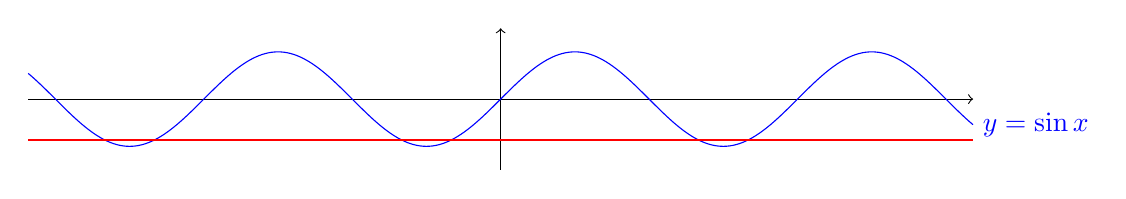
\begin{tikzpicture}[scale=0.6,samples=300]
             \draw[->] (-10,0) -- (10, 0);
             \draw[->] (0,-1.5) -- (0,1.5);
             \draw[color=blue, domain=-10:10] plot (\x,{sin(\x r)}) node[right] {$y = \sin x$};
             \draw[color=red] (-10, -0.86602540) -- (10, -0.86602540);
            \end{tikzpicture}

            $\displaystyle \sin^{-1}{\left( -\frac{\sqrt{3}}{2} \right)}$
            が表す値は赤と青の交点の$x$座標を表している為、
            次のように複数の値が存在する。
            \begin{equation}
             \frac{4\pi}{3} + 2\pi m, \  \frac{5\pi}{3} + 2\pi n
              \qquad \left( m,n \in \mathbb{Z} \right)
            \end{equation}

            関数$\sin^{-1}{x}$の値域を
            $-\frac{\pi}{2} \leq \sin^{-1}{x} \leq \frac{\pi}{2}$
            とすれば、求めるべき値は
            $\sin^{-1}{\left( -\frac{\sqrt{3}}{2} \right)}=-\frac{\pi}{3}$
            となる。


            \hrulefill

       \item
            $\displaystyle \cos^{-1}{\left( \sin{\frac{\pi}{6}} \right)}$

            \dotfill

            $\displaystyle \sin{\frac{\pi}{6}}$は一つの値のみを表しており、
            $\displaystyle \sin{\frac{\pi}{6}}=\frac{1}{2}$である。

            そこで次のグラフは、
            直線$y=\frac{1}{2}$を赤、
            曲線$y=\cos{x}$を青
            で描いたものである。

            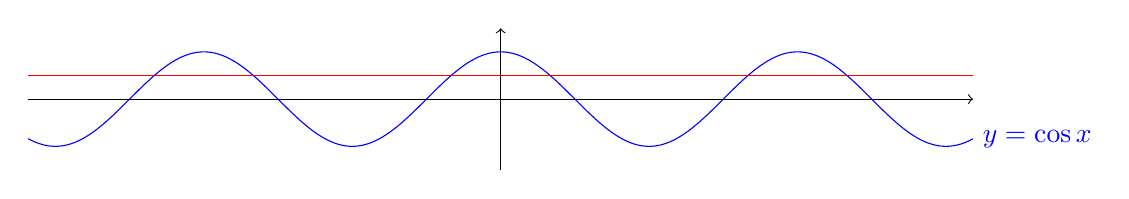
\begin{tikzpicture}[scale=0.6,samples=300]
             \draw[->] (-10,0) -- (10, 0);
             \draw[->] (0,-1.5) -- (0,1.5);
             \draw[color=blue, domain=-10:10] plot (\x,{cos(\x r)}) node[right] {$y = \cos x$};
             \draw[color=red] (-10, 0.5) -- (10, 0.5);
            \end{tikzpicture}

            よって、
            $\displaystyle \cos^{-1}{\left( \sin{\frac{\pi}{6}} \right)}$
            を満たす値は次のように複数ある。
            \begin{equation}
             \frac{\pi}{3} + 2\pi m, \  \frac{5\pi}{3} + 2\pi n
              \qquad \left( m,n \in \mathbb{Z} \right)
            \end{equation}

            関数$\cos^{-1}{x}$の値域を
            $0 \leq \cos^{-1}{x} \leq \pi$
            とすれば、求めるべき値は
            $\cos^{-1}{\left( -\frac{\sqrt{3}}{2} \right)}=\frac{\pi}{3}$
            となる。



            \hrulefill

       \item
            $\displaystyle \lim_{x\to -\infty} \tan^{-1}{x}$

            \dotfill

            $y=\tan{x}$のグラフを描くと、
            次のように
            $x=\frac{\pi}{2}n \quad (n\in\mathbb{Z})$を除いた点で
            定義される。

            \begin{tikzpicture}[scale=0.7,samples=300]
             \draw[->] (-4.34,0) -- (4.34, 0);
             \draw[->] (0,-2.7) -- (0,2.7);
             \draw[color=blue, domain=-1.2:1.2] plot ({\x, tan(\x r)});
             \draw[color=blue, domain=-4.34:-1.94] plot ({\x, tan(\x r)});
             \draw[color=blue, domain=1.94:4.34] plot ({\x, tan(\x r)});
            \end{tikzpicture}

            このグラフの原点を通る部分の
            区間$-\frac{\pi}{2} < x < \frac{\pi}{2}$
            を値域となるように
            $y=\tan^{-1}{x}$のグラフを描くと次のようになる。

            \begin{tikzpicture}[scale=1,samples=300]
             \draw[->] (-2.7,0) -- (2.7, 0);
             \draw[->] (0,-1.2) -- (0,1.2);
             \draw[color=blue, domain=-1.2:1.2] plot ({tan(\x r)}, \x) node[right] {$y = \tan^{-1} x$};
            \end{tikzpicture}

            この為、極限は次のようになる。
            \begin{equation}
             \lim_{x\to -\infty} \tan^{-1}{x}
              = -\frac{\pi}{2}
            \end{equation}

            \hrulefill

       \item
            $\displaystyle \tan^{-1}{\left(\frac{1}{2}\right)} + \tan^{-1}{\left(\frac{1}{3}\right)}$

            \dotfill

            上記グラフのように
            $\tan^{-1}{x}$の値を
            $-\frac{\pi}{2} < \tan^{-1}{x} < \frac{\pi}{2}$に制限すれば、
            $\tan^{-1}{\left(\frac{1}{2}\right)}$と
            $\tan^{-1}{\left(\frac{1}{3}\right)}$は
            一つの値となる。

            そこで、実数$a,b$を次のように置く。
            \begin{equation}
             a= \tan^{-1}{\left(\frac{1}{2}\right)}
              ,\quad
              b= \tan^{-1}{\left(\frac{1}{3}\right)}
            \end{equation}
            これにより、次のようになる。
            \begin{equation}
             \tan{a}= \frac{1}{2}
              ,\quad
              \tan{b}= \frac{1}{3}
            \end{equation}

            このとき、
            $\tan(a+b)$を求める。
            \begin{align}
             \tan(a+b)
             =
             \frac{\tan{a}+\tan{b}}{1-\tan{a}\tan{b}}
             =
             \frac{\frac{1}{2}+\frac{1}{3}}{1-\frac{1}{2}\cdot\frac{1}{3}}
             =
             1
            \end{align}

            よって、次のように求まる。
            \begin{equation}
             \tan^{-1}{\left(\frac{1}{2}\right)} + \tan^{-1}{\left(\frac{1}{3}\right)}
              = \tan^{-1}{(1)}
              = \frac{\pi}{4}
            \end{equation}

            $y=\tan^{-1}{x}$の値域を設定しないのであれば、
            直線$y=1$と曲線$y=\tan{x}$の交点から求められる。

            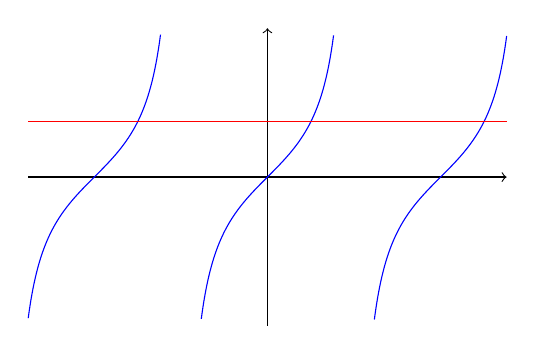
\begin{tikzpicture}[scale=0.7,samples=300]
             \draw[->] (-4.34,0) -- (4.34, 0);
             \draw[->] (0,-2.7) -- (0,2.7);
             \draw[color=blue, domain=-1.2:1.2] plot ({\x, tan(\x r)});
             \draw[color=blue, domain=-4.34:-1.94] plot ({\x, tan(\x r)});
             \draw[color=blue, domain=1.94:4.34] plot ({\x, tan(\x r)});
             \draw[color=red] (-4.34, 1) -- (4.34, 1);
            \end{tikzpicture}

            よって、次の値となる。
            \begin{equation}
             \frac{\pi}{4} + \pi n \qquad (n \in \mathbb{Z})
            \end{equation}

            \hrulefill

      \end{enumerate}

      \hrulefill
 \item
      $a,b >0,\; a,b\ne 1,\; x\in\mathbb{R}$とする。
      このとき、
      $(ab)^{x}=a^{x}b^{x}$が成り立つことを示せ。

      \dotfill

      $x\in\mathbb{R}$が有理数のとき、
      $(ab)^{x}=a^{x}b^{x}$であるので、
      $x\in\mathbb{R}$が無理数とする。

      $x$に収束する有理数のコーシー列を$\{x_{n}\}_{n\in\mathbb{N}}$とする。
      つまり、$\displaystyle \lim_{n\to\infty}x_{n}=x$である。

      各$x_{n}$は有理数であるので、
      $(ab)^{x_{n}}=a^{x_{n}}b^{x_{n}}$である。

      $\displaystyle \lim_{n\to\infty}a^{x_{n}}=a^{x},\; \lim_{n\to\infty}b^{x_{n}}=b^{x}$であることから、
      \begin{equation}
       a^{x} \times b^{x}
        =
       \lim_{n\to\infty}a^{x_{n}} \times \lim_{n\to\infty}b^{x_{n}}
       =
       \lim_{n\to\infty} (a^{x_{n}} b^{x_{n}})
      \end{equation}
      である。
      また、
      $\displaystyle \lim_{n\to\infty}(ab)^{x_{n}}=(ab)^{x}$であることから、
      $(ab)^{x_{n}}=a^{x_{n}}b^{x_{n}}$の極限を求めると
      $(ab)^{x}=a^{x}b^{x}$が得られる。

      \hrulefill

 \item
      $a>1$とする。
      このとき、$-1 < x < 0$として、
      $\displaystyle \lim_{x\to 0} a^{x} = 1$
      を証明せよ。

      \dotfill

      $0<-x<1$であるので、
      $n\leq -\frac{1}{x} <n+1$となる自然数$n$が存在する。

      $-1 \leq -\frac{1}{n} \leq x < -\frac{1}{n+1} <0$より
      \begin{equation}
       a^{-\frac{1}{n}} \leq a^{x} < a^{-\frac{1}{n+1}}
      \end{equation}
      であるので、
      数列$\{a^{-\frac{1}{n}}\}_{n\in\mathbb{N}}$と$a^{x}$の極限は一致する。
      \begin{equation}
       \lim_{n\to\infty}a^{-\frac{1}{n}}
        =\lim_{x\to 0} a^{x}
      \end{equation}

      つまり、
      $\displaystyle \lim_{n\to\infty} a^{-\frac{1}{n}}=1$
      が示せればよい。

      そこで、
      ${}^{\forall}\varepsilon > 0$としたとき
      十分に大きな$n$に対して
      $\lvert a^{-\frac{1}{n}} -1 \rvert < \varepsilon$が成り立てばよい。
      $0 < a^{-\frac{1}{n}} <1$であるので、
      絶対値を外し変形をする。
      \begin{equation}
       (1-\varepsilon)^{n} < a^{-1}
      \end{equation}

      二項定理より
      \begin{equation}
       (1-\varepsilon)^{n}
       = \sum_{i=0}^{n} {}_{n}C_{i}(-\varepsilon)^{i}
       =1 - n\varepsilon + \frac{n(n-1)}{2}\varepsilon^{2} +
       \cdots
       %+ \frac{n(n-1)}{2}(-\varepsilon)^{n-2}
       %+ n(-\varepsilon)^{n-1}
       + (-\varepsilon)^{n}
      \end{equation}
      である。

      $\lvert a^{-\frac{1}{n}} -1 \rvert < \varepsilon$が
      成立する様な状況を考えるので、
      $0<\varepsilon<1$に制限して考えても良い。

      $0<\varepsilon<1$であれば、
      \begin{equation}
       1-n\varepsilon < (1-\varepsilon)^{n} < a^{-1}
      \end{equation}
      となる。
      ここから、
      $n$は次を満たせば
      $\lvert a^{-\frac{1}{n}} -1 \rvert < \varepsilon$となる
      ことがわかる。
      \begin{equation}
       n > \frac{1}{\varepsilon}(1-a^{-1})
      \end{equation}

      これにより、
      ${}^{\forall}\varepsilon > 0$に対して、
      $\lvert a^{-\frac{1}{n}} -1 \rvert < \varepsilon$となる
      $n\in\mathbb{N}$は存在することとなり、
      $\displaystyle \lim_{n\to\infty} a^{-\frac{1}{n}}=1$
      であることがわかる。

      $\displaystyle \lim_{n\to\infty}a^{-\frac{1}{n}}=\lim_{x\to 0} a^{x}$
      であるから、
      $\displaystyle \lim_{x\to 0} a^{x}=1$
      である。

\end{enumerate}


\hrulefill

\end{document}
